% LaTeX snippets for prepared core figures/tables
% Base folder: /Users/wsun/Documents/manuscript2023/Coordinate_charts

% ---- Core best table (already generated from validated metrics) ----
% % Auto-generated by build_submission_tables.py
\begin{tabular}{lrrrrrr}
\toprule
Case & Primary & Field rel-L2 & Obs rel-L2 & $\mu$ err (\%) & $K$ err (\%) & Runtime (s)\\
\midrule
forward_poisson_ellipsoid & 0.0023 & 0.0023 & - & - & - & 106.30\\
forward_poisson_star & 0.2591 & 0.2591 & - & - & - & 229.36\\
rabbit_poisson_schwarz & 0.0221 & 0.0221 & - & - & - & 3.659e+03\\
torus_inverse_original_atlas & 2.350e-07 & - & - & 9.272e-06 & 2.289e-05 & 201.09\\
torus_inverse_schwarz_displacement & 0.0017 & - & 0.0017 & 4.083e-12 & 0.9993 & 38.63\\
torus_inverse_schwarz_traction & 0.0058 & - & 0.0058 & 0.3453 & 0.5412 & 76.89\\
rabbit_inverse_elder & 0.0300 & - & - & - & - & 12.09\\
\bottomrule
\end{tabular}


% ---- Example 1 ----
% \begin{figure}[H]
% \centering
% \includegraphics[width=0.48\textwidth]{figures_cmame_core/example1_forward_poisson/pinn_3d_ellipsoid_mapped_sphere.png}
% \includegraphics[width=0.48\textwidth]{figures_cmame_core/example1_forward_poisson/poisson_star3d_mapped_results.png}
% \caption{Forward Poisson verification on ellipsoid and star domains.}
% \label{fig:ex1_poisson}
% \end{figure}

% ---- Example 2 ----
% \begin{figure}[H]
% \centering
% 
\includegraphics[width=0.48\textwidth]{figures_cmame_core/example2_rabbit_poisson/poisson_rabbit_convergence.pdf}
% 
\includegraphics[width=0.48\textwidth]{figures_cmame_core/example2_rabbit_poisson/poisson_rabbit_error_summary.pdf}
% \caption{Rabbit Poisson Schwarz convergence and error summary.}
% \label{fig:ex2_rabbit_poisson_curves}
% \end{figure}

% ---- Example 3 ----
% \begin{figure}[H]
% \centering
% 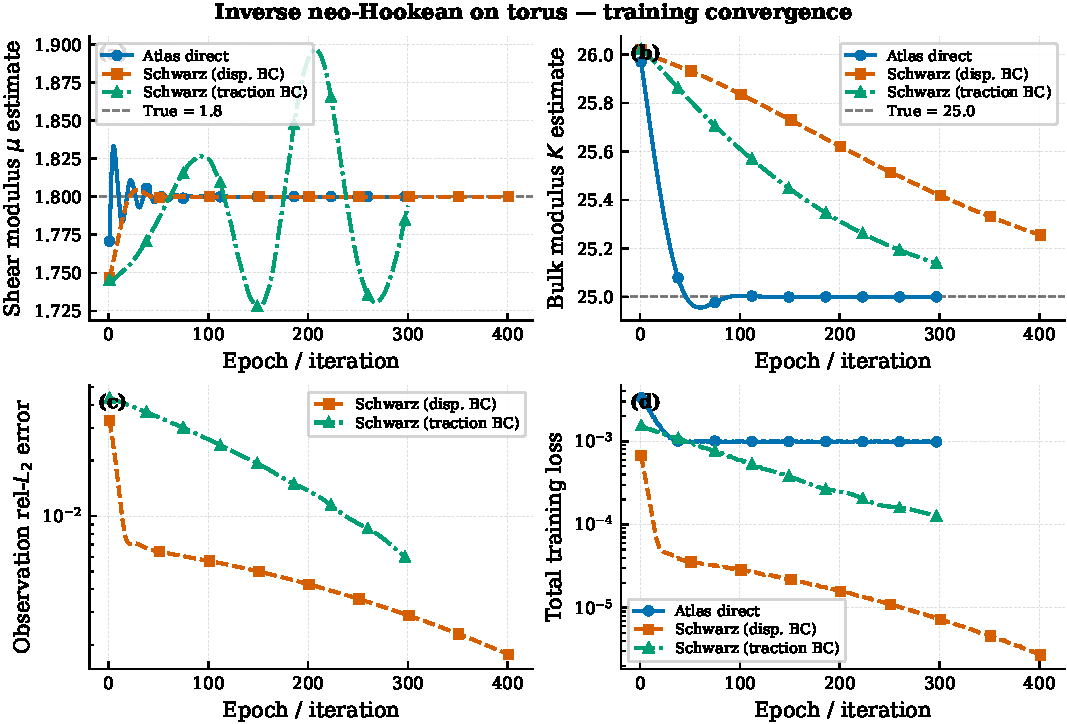
\includegraphics[width=0.48\textwidth]{figures_cmame_core/example3_torus_inverse_original/torus_inverse_convergence.pdf}
% 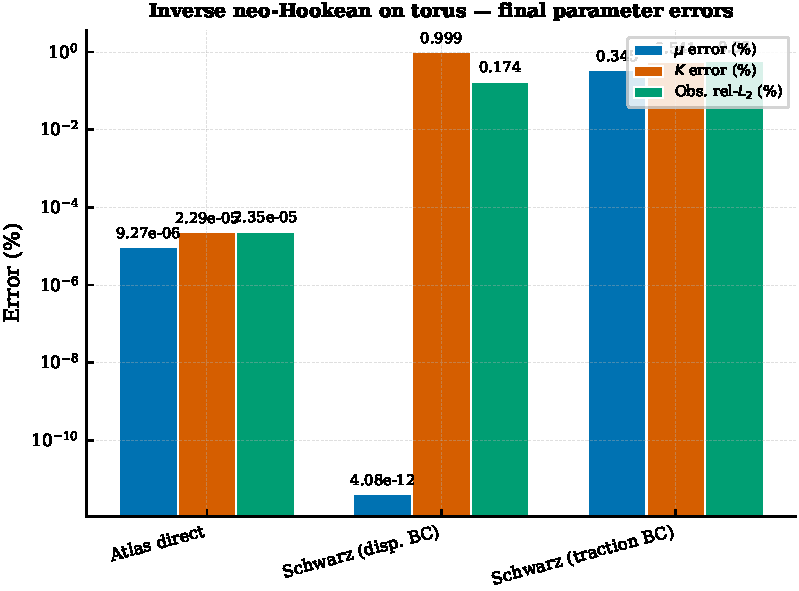
\includegraphics[width=0.48\textwidth]{figures_cmame_core/example3_torus_inverse_original/torus_inverse_summary.pdf}
% \caption{Torus inverse Neo-Hookean (original atlas): convergence and parameter summary.}
% \label{fig:ex3_torus_original}
% \end{figure}

% ---- Example 4 ----
% \begin{figure}[H]
% \centering
% \includegraphics[width=0.48\textwidth]{figures_cmame_core/example4_torus_inverse_schwarz_dual/torus_inverse_neohookean_schwarz_traction_accurate_curves.png}
% \includegraphics[width=0.48\textwidth]{figures_cmame_core/example4_torus_inverse_schwarz_dual/torus_inverse_neohookean_schwarz_displacement_accurate_curves.png}
% \caption{Torus Schwarz dual inverse (traction/displacement modes).}
% \label{fig:ex4_torus_schwarz_dual}
% \end{figure}

% ---- Example 5 ----
% \begin{figure}[H]
% \centering
% 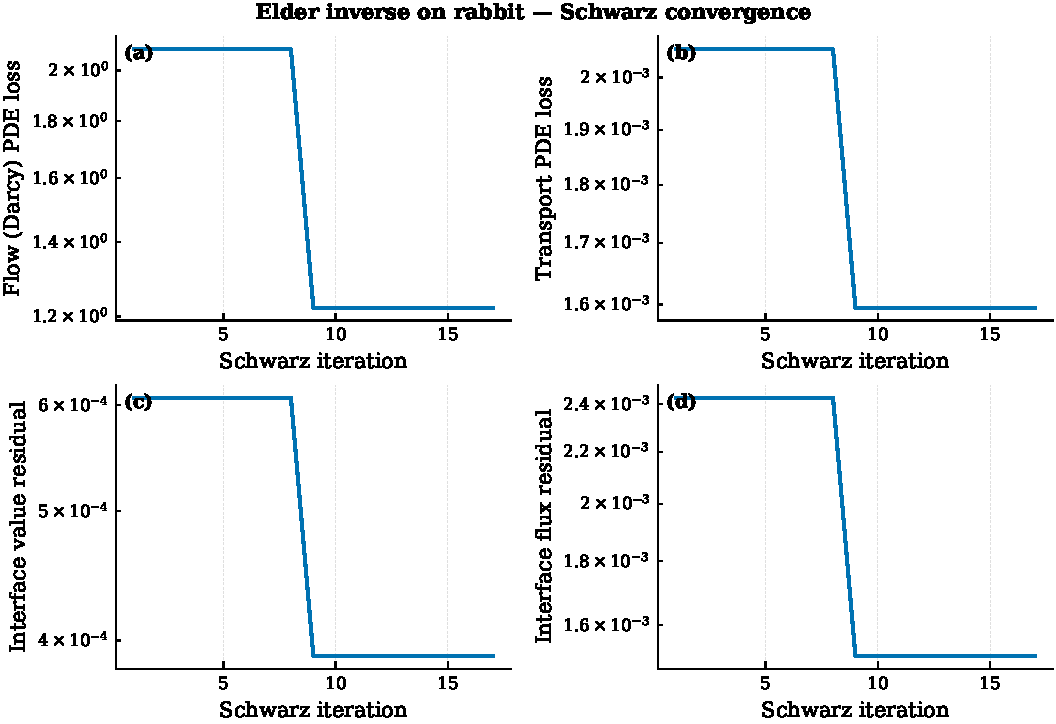
\includegraphics[width=0.48\textwidth]{figures_cmame_core/example5_rabbit_elder/elder_rabbit_convergence.pdf}
% 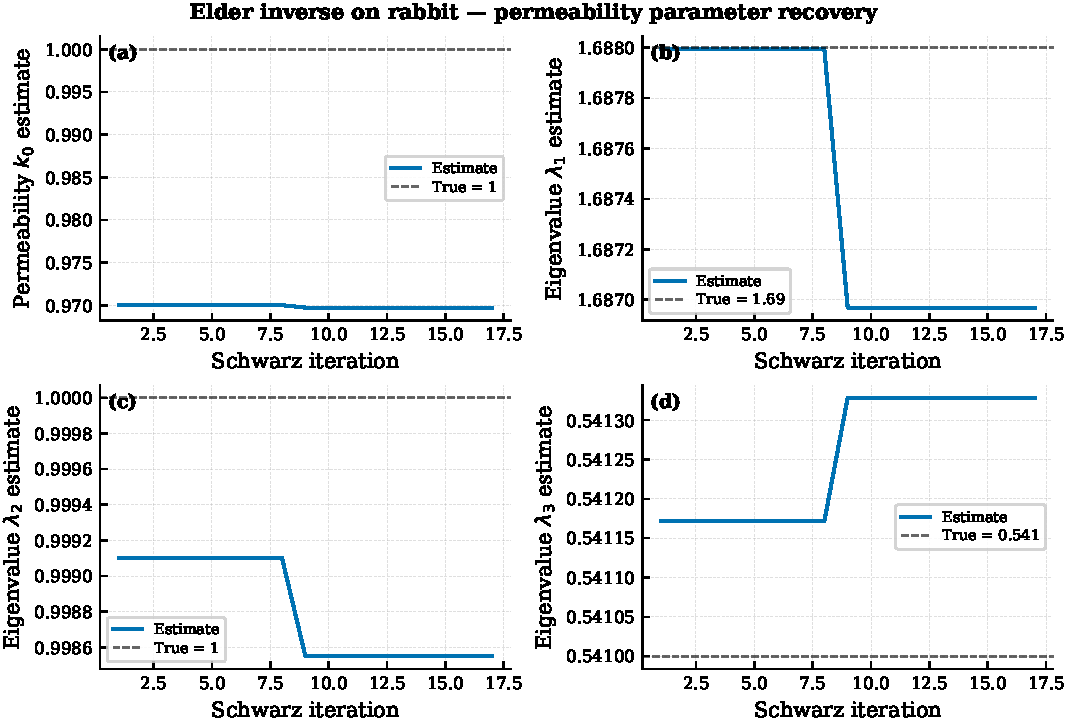
\includegraphics[width=0.48\textwidth]{figures_cmame_core/example5_rabbit_elder/elder_rabbit_parameters.pdf}
% \caption{Rabbit inverse Elder benchmark: convergence and parameter identification.}
% \label{fig:ex5_rabbit_elder}
% \end{figure}
